\documentclass[russian,utf8,emptystyle]{eskdtext}

\newcommand{\No}{\textnumero} % костыль для фикса ошибки

\ESKDdepartment{Федеральное государственное бюджетное образовательное учреждение высшего профессионального образования}
\ESKDcompany{Московский государственный технический университет им. Н. Э. Баумана}
\ESKDclassCode{23 0102}
\ESKDtitle{АИС поиска алгоритмов распознавания изоморфизма графов с помощью генетического программирования}
\ESKDdocName{Расчетно-пояснительная записка}
\ESKDauthor{Гуща~А.~В.}
\ESKDtitleApprovedBy{~}{~\underline{\hspace{2.5cm}}}
\ESKDtitleAgreedBy{~}{~\underline{\hspace{2.5cm}}}
\ESKDtitleDesignedBy{Студент группы ИУ5-82}{Гуща~А.~В}

\usepackage{multirow}
\usepackage{tabularx}
\usepackage{tabularx,ragged2e}
\usepackage{pdfpages}
\renewcommand\tabularxcolumn[1]{>{\Centering}p{#1}}
\newcommand\abs[1]{\left|#1\right|}

\usepackage{geometry}
\geometry{footskip = 1cm}

\pagenumbering{arabic}
\pagestyle{plain}

\begin{document}
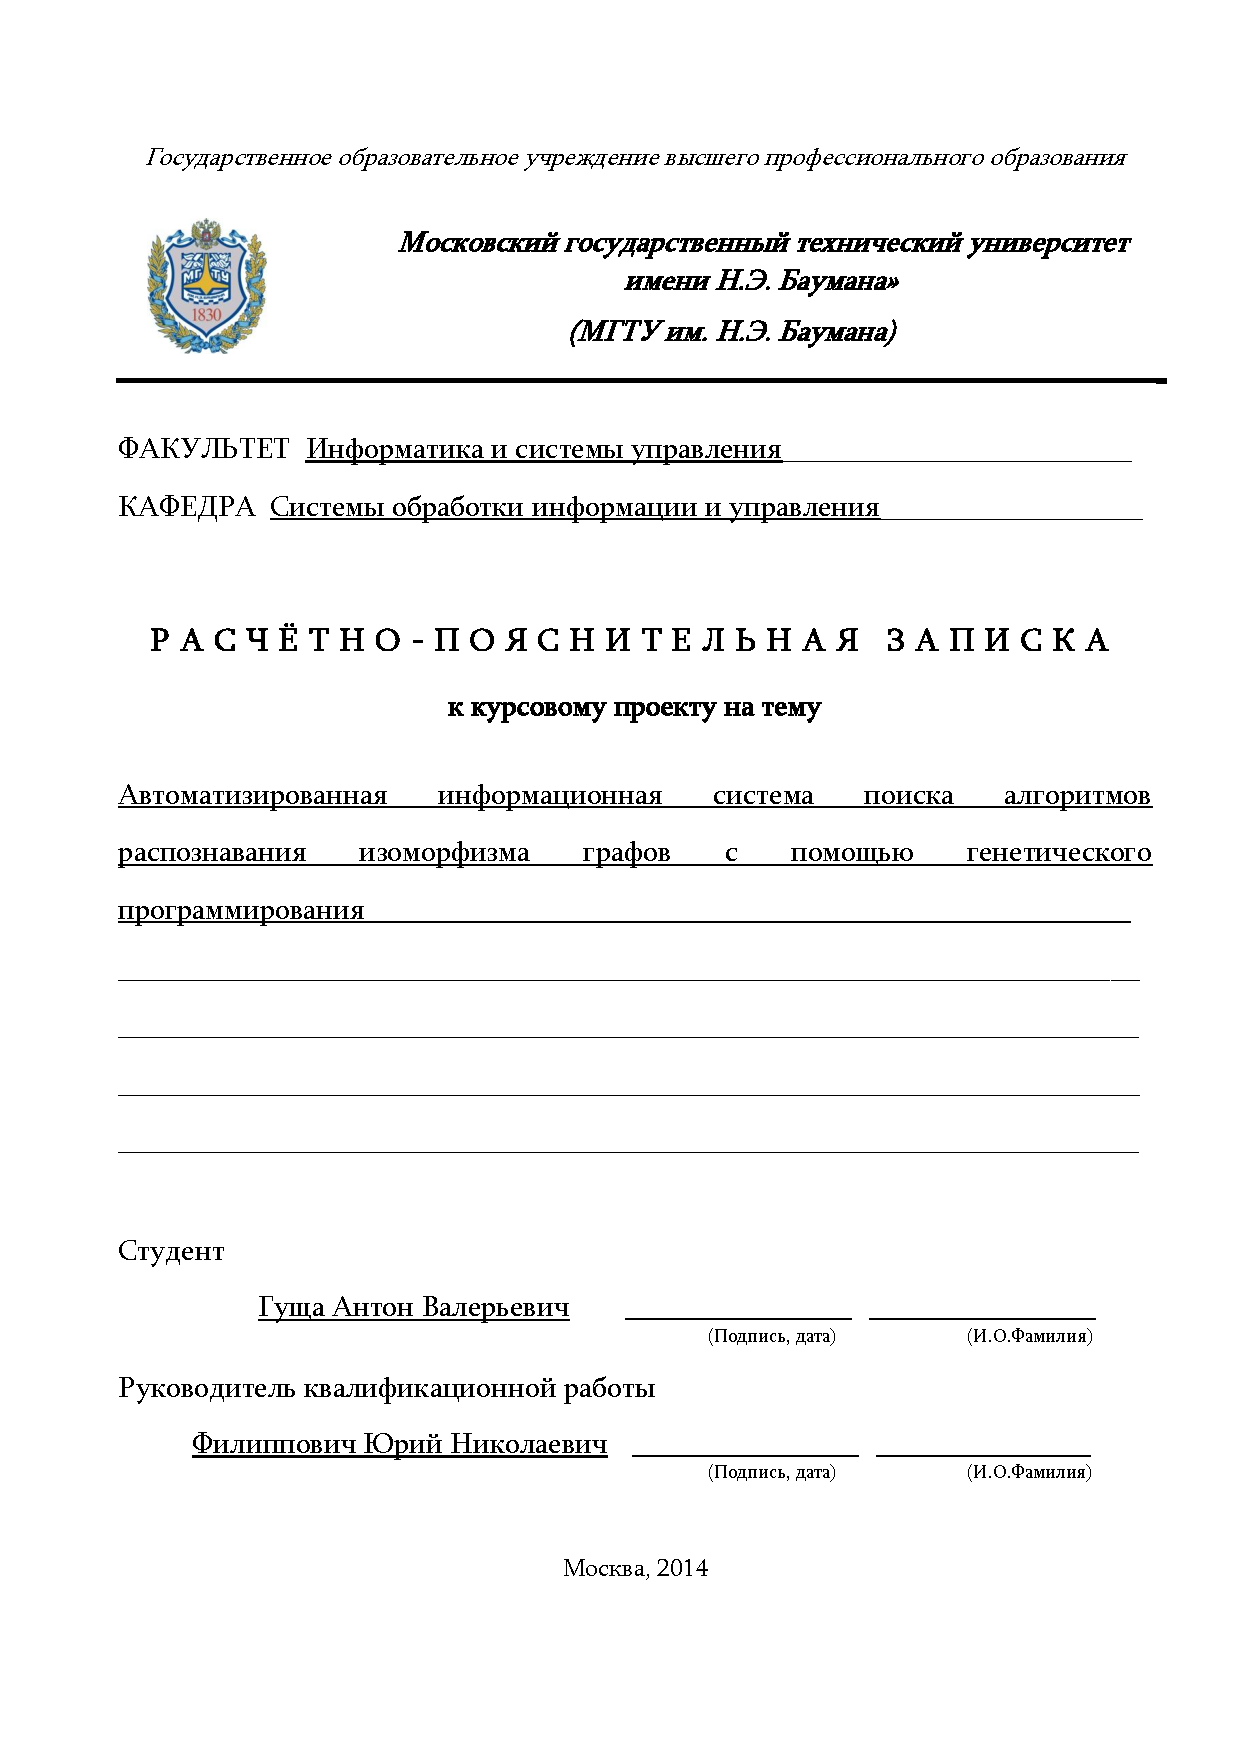
\includepdf[pages={1}]{title.pdf}

\newpage
\tableofcontents
\newpage

\section{Введение}
Задача проверки изоморфизма графов является актуальной и исключительно привлекательной проблемой в наше время. Нахождение эффективного алгоритма, который за полиномиальное время позволит отвечать на данный вопрос, положительным образом повлияет на такие прикладные задачи как:
\begin{itemize}
\item Поиск химических соединений по базам данных в хемоинформатике и математической химии
\item Верификация различных представлений электронной схемы в автоматизации проектирования электронных схем
\item Выделение общих подвыражений в оптимизации программ
\item Сопоставление графов знаний, содержащихся в семантических сетях
\end{itemize}
Уникальность данной задачи в том, что это одна из двух задач (и одна из 12, перечисленных в \cite{GareyAndJohnson1979}), для которых класс сложности не был определен. Задача проверки изоморфизма графов принадлежит классу NP задач, но не доказано, что она является NP-полной задачей, и не найден алгоритм, решающий ее за полиномиальное время.

В 60-х~--- 80-х годах неоднократно предпринимались попытки решить данную задачу, но они не увенчались успехом. На данный момент лучший алгоритм имеет временную оценку сложности $2^{O(\sqrt{n log(n)})}$ \cite{Johnson2005} \cite{BabaiCodenotti2008}.

В наши дни информационные технологии все больше используются как научные инструменты (яркий пример - решение проблемы четырех красок \cite{FourColourProblem}). С ростом вычислительной мощности растет актуальность использовать автоматические методы поиска решения, например, метод генетического программирования. В данной работе разработан инструмент, спроектированный производить поиск решения задачи проверки отношения изоморфизма для ориентированных графов с выводом преобразованных в графическую форму промежуточных результатов для анализа человеком.

\newpage
\section{Конструкторская часть}
\subsection{Общетехническое обоснование разработки}
\subsubsection{Постановка задачи проектирования}
Задача - разработать автоматизированную информационную систему, реализующую автоматический поиск алгоритмов проверки отношения изоморфизма ориентированных графов и предоставляющую графическую информацию о промежуточных результатах пользователю для анализа.

Задачи проектирования могут быть сформулированы следующим образом:
\begin{enumerate}
\item Исследование предметной области проектирования
\item Определение функциональных задач
\item Изучение метода <<Генетическое программирование>>
\item Разработка проблемно-ориентированного языка для внутреннего представления программ
\item Выбор и обоснование критериев качества программы и оценки работы найденных алгоритмов
\item Разработка схемы данных
\item Разработка алгоритмов программы
\item Разработка программы
\item Отладка программы
\item Разработка графического интерфейса пользователя
\item Тестирование программы
\item Разработка конструкторской и эксплуатационной документации
\end{enumerate}

\subsubsection{Описание предметной области}
\textbf{Ориентированный граф} - совокупность непустого множества вершин и множества связей между вершинами, называемыми ребрами. Ребра являются упорядоченными парами вершин.

\begin{align*}
G &\equiv ( E, V ) \\ 
V &\equiv \{ (e_1, e_2) | e_1 \in E \wedge e_2 \in E \}
\end{align*}

$e_1$ - \textbf{начало} ребра, $e_2$ - \textbf{конец} ребра. Далее ребро будет обозначаться следующем образом:
$$
v = e_1 \rightarrow e_2
$$
Далее рассматриваются только графы с конечным множеством вершин и ребер.

Граф $G$ называется \textbf{изоморфным} графу $H$, если существует биекция $f$ из множества вершин графа $G$ в множество вершин графа $H$, обладающая следующим свойством: если в графе $G$ есть ребро из вершины $A$ в вершину $B$, то в графе должно быть ребро из вершины $f(A)$ в вершину $f(B)$ и наоборот --- если в графе $H$ есть ребро из вершины $A$ в вершину $B$, то и в графе $G$ должно быть ребро из вершины $f^{-1}(A)$ в вершину $f^{-1}(B)$. Биекция также должна сохранять ориентацию ориентированного графа.

\begin{figure}[h!]
\centering
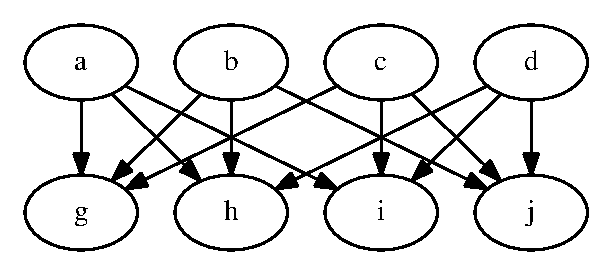
\includegraphics[scale=0.6]{graphs_isomorph_example_1}
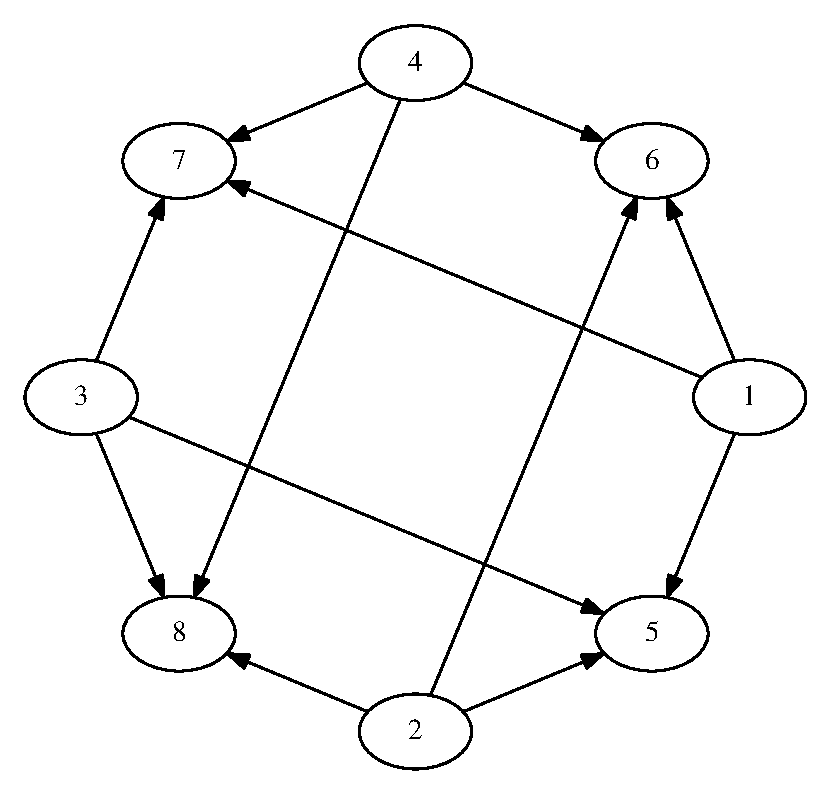
\includegraphics[scale=0.6]{graphs_isomorph_example_2}
\caption{Пример изоморфных графов}
\label{fig:graphs_isomorph_example}
\end{figure}

Пример изоморфных графов представлен на рисунке~\ref{fig:graphs_isomorph_example}.

\textbf{Матрица смежности графа $G$ с конечным числом вершин $n$} - это квадратная матрица $A$ размера $n$, в которой значение элемента $a_{ij}$ равно числу ребер из $i$-й вершины графа в $j$-ю вершину. 

Самый прямолинейный способ установить отношение изоморфности между графами $G$ и $H$ - перестановками строк и столбцов матрицы смежности графа $G$ получить матрицу смежности графа $H$. Однако перебор всех возможных перестановок характеризуется вычислительной сложностью $O(N!)$, что практически исключает применение подобного подхода на практике.

Существует набор числовых характеристик графов, называемыми полными инвариантами, совпадение которых у различных графов является необходимым и достаточным условием изоморфизма. Примерами таких инвариантов являются:
\begin{itemize}
\item Мини-код $\mu_{min}(G)$ матрицы смежности, получаемый путем выписывания двоичных значений матрицы смежности в строчку с последующим переводом полученного двоичного числа в десятичную форму. Мини-коду соответствует такой порядок следования строк и стобцов, при котором полученное значение является минимально возможным.
\item Макси-код $\mu_{max}(G)$ матрицы смежности, получаемый путем выписывания двоичных значений матрицы смежности в строчку с последующим переводом полученного двоичного числа в десятичную форму. Макси-коду соответствует такой порядок следования строк и стобцов, при котором полученное значение является максимально возможным.
\end{itemize}

В настоящее время полный инвариант графа, вычислимый за полиномиальное время, неизвестен, однако не доказано, что он не существует. Попытки его отыскания неоднократно предпринимались в 60-х~--- 80-х годах XX века, однако не увенчались успехом. На данный момент лучший алгоритм определения изоморфизма графов имеет временную оценку сложности $2^{O(\sqrt{n log(n)})}$ \cite{Johnson2005} \cite{BabaiCodenotti2008}.

\subsubsection{Перечень процессов, подлежащих автоматизации}
Процессы, которые подлежат автоматизации:
\begin{enumerate}
\item Генерация первичных алгоритмов проверки изоморфизма графов
\item Эволюционный поиск и отбор наилучших алгоритм проверки изоморфизма графов
\item Качественная оценка полученных алгоритмов проверки изоморфизма графов
\item Визуализация полученных алгоритмов проверки изоморфизма графов
\end{enumerate}

\subsubsection{Выбор и обоснование критериев качества}
Для проектируемой автоматизированной информационной системы приоритетными являются следующие критерии качества:
\begin{itemize}
\item скорость обработки эволюционного процесса
\item используемая память во время обработки эволюционного процесса
\item лицензия на исходный код и исполняемые файлы
\item стоимость приобретения или использования программного продукта
\item используемый язык программирования
\item используемый подход для представления исходного кода алгоритмов
\item удобство работы и документация
\end{itemize}

\textbf{Скорость обработки эволюционного процесса} - однозначно определяется временем, затрачиваемым на обработку одного поколения индивидов при одинаковом количестве запусков на каждого индивида и настройках эволюционных операторов. Данный параметр является самым важным, он определяет насколько быстрее программный продукт найдет качественные решения.

\textbf{Используемая память во время обработки эволюционного процесса} - определяется эффективностью использования адресного пространства ОЗУ вычислительного средства. Меньшее потребление памяти позволяет запускать большее число параллельных популяций для поиска алгоритмов. Является менее важным параметром, так как при плохой скорости обработки преимущество в используемой памяти несущественно.

\textbf{Лицензия на исходный код и исполняемые файлы} - лицензии регулируют правила пользования исходными кодами программы и исполняемыми файлами. Преимущество дают широко распространенные \textbf{свободные} лицензии, котырые позволяют просматривать, модифицировать и распрострянять исходные коды, а к исполняемым файлам прикрепляется инструкция получения исходных кодов. Закрытые (проприетарные) лицензии зачастую используются в платном программном обеспечении, что резко ограничивает его применимость.

\textbf{Стоимость приобретения или использования программного продукта} - многие программные продукты спроектированы для профессионального и/или коммерческого использования, и разработчики данных программ требуют оплату при получении или использовании их программ.

\textbf{Используемый язык программирования} - необходимо разработать АИС на языке программирования \textbf{D}, который является на данный момент современным языком системного и прикладного программирования, ориентированный на создание эффективных понятных и крупных программных комплексов. Пополнение и использование экосистемы языка \textbf{D} является значительным вкладом в развитие области. Для использования других языков с программами, написанными на \textbf{D}, необходимо наличие C-API или специальной обертки, которая пишется программистом под собственные нужды, что означает дополнительные расходы. Поэтому системы, написанные на других языках и которые имеют C-API рассматриваются как более удобные, чем без данного интерфейса взаимодействия.

\textbf{Используемый подход для представления исходного кода алгоритмов} - различные системы генетического программирования используют различные способы представления исходного кода алгоритмов. Для решения рассматриваемой задачи древовидный подход оценивается как самый удобный, так как в процессе эволюции создаются целые алгоритмы, что отличает генетическое программирование от генетических алгоритмов и похожих методов.

\textbf{Удобство работы и документация} - для работы с автоматизированными информационными системами, являющимися научными инструментами, необходимы общирная документация и удобство работы, чтобы обеспечить наискорейшее получение результатов. 

\begin{table}
\centering
\caption{Принятые значения весовых коэффициентов}
\label{tab:quality_koeff}
\begin{tabular}{c|c|c}
Коэффициент & Значение & Описание \\ 
\hline 
$K_1$ & 0.2 & Скорость обработки \\ 
\hline 
$K_2$ & 0.1 & Используемая память \\ 
\hline 
$K_3$ & 0.15 & Лицензия \\ 
\hline 
$K_4$ & 0.15 & Стоимость \\ 
\hline 
$K_5$ & 0.3 & Язык программирования \\ 
\hline 
$K_6$ & 0.05 & Представление алгоритма \\ 
\hline 
$K_7$ & 0.05 & Удобство работы и документация 
\end{tabular} 
\end{table}

Итоговые значения весовых коэффициентов для метода базового критерия представлены в таблице~\ref{tab:quality_koeff}. Необходимое для метода базового критерия нормировки соблюдено:
$$
\sum_i K_i = 1
$$

\subsubsection{Анализ аналогов и прототипов}
Генетическое программирование было заложено Koza, J.R. в \cite{KozaTheBase} в 1992 году. С того времени появилось немало реализаций данного метода, но для сравнения были выбраны самые используемые и широко распространенные.

\paragraph{JGAP} - библиотека, написанная на языке Java, для генетического программирования и генетических алгоритмов. Она предоставляет базовые генетические механизмы, которые могут быть легко использованы в эволюционном подходе для решений задач. JGAP спроектирована простой для использования "из коробки", при этом являясь гибкой системой для того, чтобы пользователи могли легко добавлять свои генетические операторы и другие компоненты.

Документация, качество и стабильность кода являлись главными критериями при проектировании JGAP. Исходный код содержит множество тестов, документирующие комментарии и множество примеров.

Преимущества:
\begin{itemize}
\item Отличная документация и удобство пользования
\item Открытая лицензия
\item Бесплатность
\item Использование необходимой модели внутреннего языка
\end{itemize}

Недостатки:
\begin{itemize}
\item Большое использование памяти (особенность языка)
\item Использование языка, требующего трудоемкой разработки обертки 
\end{itemize}

\paragraph{ECJ} - исследовательская система, написанная на языке Java. Имеет крайне гибкую структуру, где все классы загружаются во время исполнения по заданным пользователем конфигурационным файлам. Также данная система разработана с учетом высокой производительности вычислений.

Преимущества:
\begin{itemize}
\item Высокая скорость обработки
\item Открытая лицензия
\item Бесплатность
\item Использование необходимой модели внутреннего языка
\end{itemize}

Недостатки:
\begin{itemize}
\item Большое использование памяти (особенность языка)
\item Использование языка, требующего трудоемкой разработки обертки 
\item Недостаточный объем документации и примеров
\end{itemize}

\paragraph{ECF} - библиотека, написанная на языке C++, предназначенная для моделирования любого вида эволюционных вычислений. Включает в себя широкий набор методов эволюционных оптимизаций, многопоточное исполнение, хорошо конфигурируемый процесс эволюции.

Преимущества:
\begin{itemize}
\item Высокая скорость обработки
\item Открытая лицензия
\item Бесплатность
\end{itemize}

Недостатки:
\begin{itemize}
\item Использование языка, требующего разработки обертки 
\item Недостаточный объем документации и примеров
\item Используется неудобный способ представления алгоритмов
\end{itemize}

\paragraph{Discipulus} - коммерческая система генетического программирования. Предположительно написанна на C\#, заявляется удобство представления входных данных, интеллектуальная система настройки эволюционного процесса и встроенная защита от проблемы, называемой <<переобучение>>.

Преимущества:
\begin{itemize}
\item Имеет C-API, не нужна разработка обертки
\item Заявляется удобство использования, отсутствующее у конкурентов
\end{itemize}

Недостатки:
\begin{itemize}
\item Платность
\item Проприетарная лицензия
\item Недостаточный объем документации и примеров
\item Мало информации о системе
\end{itemize}

\paragraph{Самостоятельно разработанная АИС} - использован языке программирования \textbf{D}, используется гибкая система, позволяющая заменять любой компонет системы и добавлять свои генетические операции. Предусмотрено множество параметров системы, которые доступны для регулирования пользователем. Система разработана с учетом необходимости высокой производительности и низкого потребления памяти.

Преимущества:
\begin{itemize}
\item Высокая скорость обработки
\item Низкое потребление памяти
\item Написана на целевом языке, не требует оберток
\item Открытая лицензия
\item Бесплатность
\item Большой объем документации различных видов
\end{itemize}

Недостатки:
\begin{itemize}
\item Проблемы со стабильность из-за малого срока разработки
\item Узкая заточенность под конкретную задачу
\end{itemize}

Перевод качественных параметров в количественные производится при помощи таблицы~\ref{tab:quality_to_value}.
\begin{table}
\centering
\caption{Таблица перевода качественных параметров в количественные}
\label{tab:quality_to_value}
\begin{tabular}{|c|c|c|c|c|}
\hline 
Качественное значение & Отлично & Хорошо & Удовлетворительно & Плохо \\ 
\hline 
Количественное значение & 1 & 0.8 & 0.5 & 0.2 \\ 
\hline 
\end{tabular} 
\end{table}

Сперва сравним аналоги без учета весовых коэффициентов, результат сравнения представлен в таблице~\ref{tab:analog_compare_phase1}. Приведенные и нормированные значения количественных критериев с учетом весовых коэффициентов представлены в таблице~\ref{tab:analog_compare_phase2}.

\begin{table}
\centering
\caption{Сравнение аналогов без перевода в количественные значения}
\label{tab:analog_compare_phase1}
\begin{tabular}{c|c|c|c|c|c}
Критерий & JGAP & ECJ & ECF & Discipulus & Данная АИС \\ 
\hline 
$K_1$ & Отлично & Хорошо & Отлично & Хорошо & Хорошо \\ 
\hline 
$K_2$ & Удовл. & Удовл. & Хорошо & Хорошо & Хорошо \\ 
\hline 
$K_3$ & Отлично & Отлично & Отлично & Удовл. & Отлично \\ 
\hline 
$K_4$ & Отлично & Отлично & Отлично & Плохо & Отлично \\ 
\hline 
$K_5$ & Удовл. & Удовл. & Хорошо & Хорошо & Отлично \\ 
\hline 
$K_6$ & Отлично & Отлично & Хорошо & Хорошо & Отлично \\ 
\hline 
$K_7$ & Отлично & Удовл. & Удовл. & Плохо & Хорошо 
\end{tabular} 
\end{table}

\begin{table}
\centering
\caption{Сравнение аналогов и прототипов с учетом нормировки и весовых коэффициентов}
\label{tab:analog_compare_phase2}
\begin{tabular}{c|c|c|c|c|c|c}
Критерий & $\alpha$ & JGAP & ECJ & ECF & Discipulus & Данная АИС \\ 
\hline 
$K_1$ & 0.2 & 1.0 & 0.8 & 1.0 & 0.8 & 0.8 \\ 
\hline 
$K_2$ & 0.1 & 0.5 & 0.5 & 0.8 & 0.8 & 0.8 \\ 
\hline 
$K_3$ & 0.15 & 1.0 & 1.0 & 1.0 & 0.5 & 1.0 \\ 
\hline 
$K_4$ & 0.15 & 1.0 & 1.0 & 1.0 & 0.2 & 1.0 \\ 
\hline 
$K_5$ & 0.3 & 0.5 & 0.5 & 0.8 & 0.8 & 1.0 \\ 
\hline 
$K_6$ & 0.05 & 1.0 & 1.0 & 0.8 & 0.8 & 1.0 \\ 
\hline 
$K_7$ & 0.05 & 1.0 & 0.5 & 0.5 & 0.2 & 0.8 \\ 
\hline 
$\sum_i \alpha_i K_i$ & 1.0 & 0.8 & 0.735 & 0.885 & 0.635 & 0.93  
\end{tabular} 
\end{table}

Из произведенных расчетов видно, что разработка собственной информационной автоматизированной системы является целесообразным, так как она соответствует поставленным целям лучше, чем существующие аналоги.

\newpage
\subsection{Разработка программного изделия}
\subsubsection{Разработка структуры программного изделия}
АИС состоит из нескольких подсистем и разбита на две большие части:
\begin{itemize}
\item Внутренняя часть, которая разрабатывалась специально под решаемую задачу в рамках данной работы. Модули, относящиеся к этой части, будем называть \textbf{внутренние}. 
\item Внешняя часть - модули, относящиеся к библиотеке генетического программирования \textbf{Devol}, разработанной ранее как многофункциональное инструментальное средство для генетического программирования. Изначально \textbf{Devol} являлся коллективной разработкой (автор является одним из основных разработчиков), и в рамках данной работы эта библиотека была переработана и дополнена, чтобы отвечать поставленным целям. Данные модули будем называть \textbf{внешние}.
\end{itemize}

Графическая схема модулей АИС представлена на листе~2 графической части.

\subsubsection{Описание модулей программного изделия}
Внутренние модули АИС:
\begin{itemize}
\item \textbf{main} - главный модуль системы, точка входа приложения. В нем инициализируются объект приложения, все окна и логгер
\item \textbf{application} - описание класса приложения, хранит ссылки на все окна, логгер, проект и управляет механизмом завершения работы приложения
\item \textbf{project} - описание сохраняемых параметров АИС. Сохранению подлежат: параметры эволюции, имя популяции и популяция
\item \textbf{gui} - пакет, который содержит подпакеты, относящиеся к графическому интерфейсу пользователя:
\begin{itemize}
\item \textbf{evolution} - описание окна эволюции
\item \textbf{generic} - описание общего поведения для всех окон, включая главное меню
\item \textbf{results} - описание окна результатов
\item \textbf{settings} - описание окна настроек эволюции и просмотра проблемно-ориентированного языка
\item \textbf{util} - содежрит алгоритм переключения между окнами
\end{itemize}
\item \textbf{graph} - пакет, содержащий подпакеты, относящиеся к реализации ориентированных графов:
\begin{itemize}
\item \textbf{connectivity} - реализация ориентированного графа на списках связности
\item \textbf{directed} - описание интерфейса ориентированного графа
\end{itemize}
\item \textbf{evol} - пакет, содержащий подпакеты, относящиеся к эволюционным процессам:
\begin{itemize}
\item \textbf{compiler} - описание стратегии компиляции, параметризация популяции и интерпретатора проблемно-ориентированного языка
\item \textbf{individ} - описание алгоритма распознавания изоморфизма графов как инидивида в популяции
\item \textbf{progtype} - описание настроек эволюционного процесса, также загружает все операторы и типы проблемно-ориентированного языка
\item \textbf{world} - описание среды, в которой выполняются программы-индивиды. Описание функции приспособленности и генерации входных графов
\item \textbf{operators} - пакет, содержащий подпакеты, относящиеся к операторам проблемно-ориентированного языка:
\begin{itemize}
\item \textbf{and} - описание оператора логического "И"
\item \textbf{answer} - описание оператора записи ответа на поставленную задачу
\item \textbf{construct} - описание создание аргумента, описывающего ребро графа
\item \textbf{dist} - описание получения индекса конца ребра графа
\item \textbf{div} - описание арифметического оператора деления
\item \textbf{gdup} - описание операции над стеком общего назначения: дублирование вершины стека
\item \textbf{gover} - описание операции над стеком общего назначения: копирование аргумента под вершиной стека и расположение копии на вершине
\item \textbf{gpop} - описание операции над стеком общего назначения: снятие значения с вершины стека
\item \textbf{gpush} - описание операции над стеком общего назначения: сохранение аргумента в стеке
\item \textbf{grot} -  описание операции над стеком общего назначения: перемещение третьего с вершины аргумента в стеке на вершину
\item \textbf{gswap} - описание операции над стеком общего назначения: перемещение вершины стека под следующий за ней аргумент
\item \textbf{idcast} -  описание оператора преобразования целочисленной переменной в действительную
\item \textbf{idup} - описание операции над входными стеками: дублирование вершины стека
\item \textbf{iover} - описание операции над входными стеками: копирование аргумента под вершиной стека и расположение копии на вершине
\item \textbf{ipop} - описание операции над входными стеками: снятие значения с вершины стека
\item \textbf{ipush} - описание операции над входными стеками: сохранение аргумента в стеке
\item \textbf{irot} -  описание операции над входными стеками: перемещение третьего с вершины аргумента в стеке на вершину
\item \textbf{iswap} - описание операции над входными стеками: перемещение вершины стека под следующий за ней аргумент
\item \textbf{mult} - описание арифметического оператора умножения
\item \textbf{not} -  описание оператора логичекого "НЕ"
\item \textbf{opif} - описание оператора логического вевтления
\item \textbf{opwhile} - описание оператора цикла
\item \textbf{or} - описание оператора логического "ИЛИ"
\item \textbf{plus} - описание оператора арифметического сложения
\item \textbf{relation} - описание операторов сравнения: больше, меньше, больше равно, меньше равно
\item \textbf{round} - описание оператора округления, преобразования действительного аргумента к целочисленному
\item \textbf{source} - описание получения индекса начала ребра графа
\end{itemize}
\item \textbf{types} - пакет, содержащий подпакеты, относящиеся к описанию типов проблемно-ориентированного языка:
\begin{itemize}
\item \textbf{argedge} - описание аргумента, содержащего ребро графа
\item \textbf{typedge} - описание типа ребра графа
\end{itemize}
\end{itemize}
\end{itemize}

Внешние модули АИС, используемые во внутренних модулях:
\begin{itemize}
\item \textbf{devol.compiler} - описание общих процедур интерпретации программ-индивидов
\item \textbf{devol.population} - описание популяции-контейнера, параметризируемого пользовательским типом инидивидов
\item \textbf{devol.individ} - описание базовой абстракции индивида-программы, перегружаемой пользователем
\item \textbf{devol.std.argvoid} - описание аргумента "нулевого" типа
\item \textbf{devol.programtype} - описание необходимых параметров, которые должен предоставить пользователь для работы эволюционного процесса
\item \textbf{devol.operatormng} - менеджер операторов, хранящий в себе все операторы проблемно-ориенитированного языка
\item \textbf{devol.operator} - базовое описание оператора, которое должен перегружать пользователь для создания своих операторов
\item \textbf{devol.std.typepod} - описание типа, содержащего простые типы данных
\item \textbf{devol.std.argpod} - описание аргумента, содержащего значения простых типов данных
\item \textbf{devol.world} - базовое описание окружения, которое пререгружается пользователем
\item \textbf{devol.argument} - описание аргумента, хранящего значения некоторого типа
\item \textbf{devol.type} - описание типа, используемого в операторах проблемно-ориенитрованного языка
\item \textbf{devol.serializable} - интерфейс, стандартизирующий операции сохранения/загрузки
\item \textbf{devol.typemng} - менеджер типов, хранящий все типы, используемые в проблемно-ориентированном языке
\end{itemize}

\subsubsection{Особенности выбранных технологий}
Все компоненты АИС написаны на языке программирования \textbf{D}, используются следующие зависимости:
\begin{itemize}
\item gtk-d - привязки к библиотеке графических элементов GTK+
\item dyaml - пакет, реализующий операции сохранения и загрузки и/в формат YAML
\item devol - разработанный автором пакет для генетического программирования
\end{itemize}

\subsubsection{Язык програмирования D}
\textbf{D} — объектно-ориентированный, императивный, мультипарадигмальный язык программирования, созданный Уолтером Брайтом из компании Digital Mars. Изначально был задуман как переработка языка C++, однако, несмотря на значительное влияние С++, не является его вариантом. В D были заново реализованы некоторые свойства C++, также язык испытал влияние концепций из других языков программирования, таких как Java, Python, Ruby, C\# и Eiffel.

При создании языка D была сделана попытка соединить производительность компилируемых языков программирования с безопасностью и выразительностью динамических. Код на языке D обычно работает так же быстро как эквивалентный код на C++, при этом программа на D короче и обеспечивает безопасный доступ к памяти.

D является мультипарадигменным языком и поддерживает в полной мере следующие парадигмы:
\begin{itemize}
\item процедурно-структурное программирование
\item объектно-ориентированное программирование
\item функциональное программирование
\item контрактное программирование
\item обобщенное программирование
\end{itemize}

D получает все большую популярность из-за преимуществ над предшественником C++. Развитая система обобщенного программирования с переосмысленными шаблонами и примесями вместе с интроспекцией дает мощный инструмент для создания эффективных и гибких приложений, работающих под разными платформами. В D присутствует выполенение функций на этапе компиляции, что позволяет "программировать" компилятор и определять свои проблемно-ориентированные языки.

D используеют сборщик мусора, который можно отключить для тех частей приложения, для которых необходимо ручное управление памятью. 

Объектно-ориентированная парадигма языка D является продолжателем идей, заложенных в С++ и развитых в языке Java, но имеет свои особенности. Так, например, классы передаются в функции только по ссылке, без изначально заложенной возможности копирования по значению. В языке отсутствует множественное наследование классов, но имеется множественное наследование интерфесов.

\subsubsection{Язык разметки YAML}
\textbf{YAML} — человекочитаемый формат сериализации данных, концептуально близкий к языкам разметки, но ориентированный на удобство ввода-вывода типичных структур данных многих языков программирования. Используется в АИС для сохранения информации о проекте.

\subsubsection{Библиотека графических элементов GTK+}
\textbf{GTK+} (сокращение от GIMP ToolKit) — кроссплатформенная библиотека элементов интерфейса, имеет простой в использовании API, наряду с Qt является одной из двух наиболее популярных на сегодняшний день библиотек для X Window System. Используется в АИС для построения графического интерфейса пользователя.

\subsubsection{Архитектруа программы. UML-диаграмма классов}
Во время проектирования приложения были выбраны следующие директивы:
\begin{itemize}
\item Максимальная гибкость. Архитектура приложения должна поддерживать легкое изменение практически всех компонентов, включая добавление и удаление новых типов и операторов проблемно-ориентированного языка
\item Максимальная эффективность. Используя богатые возможности языка D, программа должна выполняться как можно быстрее и потреблять как можно меньше памяти, при этом не терять в гибкости и скорости разработки
\item Минимальные издержки. Все операции, которые могут быть проведены и верифицированы на этапе компиляции, должны быть перемещены на этап компиляции. Критически важные алгоритмы должны быть протестированы встроенными модульными тестами.
\end{itemize}

Классы, используемые в АИС, можно разделить на 3 типа:
\begin{itemize}
\item Ядро - классы, обеспечивающие описание графов, приложения и логики сохранения/загрузки информации
\item Графический интерфейс - классы, описывающие графический интерфейс пользователя
\item Эволюционные - описание внутреннего проблемно-ориентированного языка генетического программирования
\item Внешние - используемые зависимости и классы библиотеки Devol
\end{itemize}

Диаграмма классов изображена на листе 6 графической части.

Перечень классов:
\begin{itemize}
\item \textbf{Application} - содержит проект и все окна приложения, определяет алгоритмы инициализации и завершения работы приложения
\item \textbf{Project} - проект, хранящий все параметры эволюционного процесса, имя популяции и последнюю найденную популяцию
\item \textbf{EvolutionWindow} - окно эволюции, в котором отображается процесс эволюции
\item \textbf{GenericWindow} - хранит в себе общее поведение для всех окон, включая главное меню
\item \textbf{ResultsWindow} - окно результатов, в котором отображаются индивиды текущей популяции
\item \textbf{SettingsWindow} - окно настроек эволюции, где пользователь может просмотреть используемые операторы и настроить процесс эволюции
\item \textbf{IDirectedGraph} - интерфейс, описывающий ориентированный граф
\item \textbf{ConnListGraph} - реализация ориентированного графа на основе списков смежности
\item \textbf{GraphWorld} - описание окружения исполнения алгоритмов проверки изоморфизма, отвечает за генерацию входных графов
\item \textbf{ProgramType} - описание параметров эволюционного процесса, все настройки эволюции находятся в этом классе
\item \textbf{GraphIndivid} - описание алгоритма проверки изоморфизма графов как индивида в популяции. Каждый индивид содержит в себе три стека:
\begin{itemize}
\item Стек общего назначения с действительным типом элементов
\item Первый входной стек для первого графа
\item Второй входной стек для второго графа
\end{itemize}
\item \textbf{GraphPopulation} - контейнер для индивидов, параметризированный типом GraphIndivid
\item \textbf{GraphCompilation} - описание правил компиляции индивидов и популяций. Является наследником GamePopulation, использующий раундовый метод определения итогового значения функции приспособленности.
\item \textbf{GraphCompiler} - интерпретатор алгоритмов в терминах проблемно-ориентированного языка для популяций GraphIndivid со стандартными алгоритмами мутации, кросинговера, нахождения нужных поддеревьев над типизированными деревьями.
\item \textbf{TypeEdge} - описание типа ребра графаф для внутреннего языка, является упорядоченной парой индексов вершин
\item \textbf{ArgEdge} - описание контейнера для значения типа ребра графа
\item \textbf{AndOperator} - описание оператора логического "И"
\item \textbf{AnswerOperator} - описание оператора записи ответа на поставленную задачу
\item \textbf{ConstructOperator} - описание создание аргумента, описывающего ребро графа
\item \textbf{DistOperator} - описание получения индекса конца ребра графа
\item \textbf{DivOperator} - описание арифметического оператора деления
\item \textbf{GenericDupOperator} - описание операции над стеком общего назначения: дублирование вершины стека
\item \textbf{GenericoverOperator} - описание операции над стеком общего назначения: копирование аргумента под вершиной стека и расположение копии на вершине
\item \textbf{GenericpopOperator} - описание операции над стеком общего назначения: снятие значения с вершины стека
\item \textbf{GenericpushOperator} - описание операции над стеком общего назначения: сохранение аргумента в стеке
\item \textbf{GenericrotOperator} -  описание операции над стеком общего назначения: перемещение третьего с вершины аргумента в стеке на вершину
\item \textbf{GenericswapOperator} - описание операции над стеком общего назначения: перемещение вершины стека под следующий за ней аргумент
\item \textbf{IntDoubleCastOperator} -  описание оператора преобразования целочисленной переменной в действительную
\item \textbf{InputDupFirstOperator, InputDupSecondOperator} - описание операции над входными стеками: дублирование вершины стека
\item \textbf{InputOverFirstOperator, InputOverSecondOperator} - описание операции над входными стеками: копирование аргумента под вершиной стека и расположение копии на вершине
\item \textbf{InputPopFirstOperator, InputPopSecondOperator} - описание операции над входными стеками: снятие значения с вершины стека
\item \textbf{InputPushFirstOperator, InputPushSecondOperator} - описание операции над входными стеками: сохранение аргумента в стеке
\item \textbf{InputRotFirstOperator, InputRotSecondOperator} -  описание операции над входными стеками: перемещение третьего с вершины аргумента в стеке на вершину
\item \textbf{InputSwapFirstOperator, InputSwapSecondOperator} - описание операции над входными стеками: перемещение вершины стека под следующий за ней аргумент
\item \textbf{MultOperator} - описание арифметического оператора умножения
\item \textbf{NotOperator} -  описание оператора логичекого "НЕ"
\item \textbf{IfOperator} - описание оператора логического вевтления
\item \textbf{WhileOperator} - описание оператора цикла
\item \textbf{OrOperator} - описание оператора логического "ИЛИ"
\item \textbf{PlusOperator} - описание оператора арифметического сложения
\item \textbf{IntEqualOperator} - описание оператора равенства целочисленных значений
\item \textbf{DoubleEqualOperator} - описание оператора равенства действительных значений
\item \textbf{IntGreaterOperator} - описание оператора "больше" для целочисленных значений
\item \textbf{IntLesserOperator} - описание оператора "меньше" для целочисленных значений
\item \textbf{IntGreaterEqualOperator} - описание оператора "больше равно" для целочисленных значений
\item \textbf{IntLesserEqualOperator} - описание оператора "меньше равно" для целочисленных значений
\item \textbf{DoubleGreaterOperator} - описание оператора "больше" для действительных значений
\item \textbf{DoubleLesserOperator} - описание оператора "меньше" для действительных значений
\item \textbf{DoubleGreaterEqualOperator} - описание оператора "больше равно" для действительных значений
\item \textbf{DoubleLesserEqualOperator} - описание оператора "меньше равно" для действительных значений
\item \textbf{RoundOperator} - описание оператора округления, преобразования действительного аргумента к целочисленному
\item \textbf{SourceOperator} - описание получения индекса начала ребра графа
\item \textbf{ProgramTypeAbstract} - базовое описание параметров, которые должны быть заданы для эволюционного процесса
\item \textbf{IndAbstract} - базовое описание индивида, которое должно быть задано для эволюционного процесса
\item \textbf{Individ} - стандартная реализация индивида, которое перегружается пользователем для описания своих индивидов
\item \textbf{WorldAbstract} - базовое описание окружения исполнения индивида
\item \textbf{ILogger} - интерфейс для системы логгирования. Конкретная реализация скрыта за этим интерфейсом.
\item \textbf{GameCompilation} - базовое описание стратегии компиляции "игра"
\item \textbf{Singleton} - описание свойств объекта, который существует только в одном экземпляре
\item \textbf{Evolutor} - содержит описание эволюционных алгоритмов
\item \textbf{PopAbstract} - базовое описание контейнера для инидвидов
\item \textbf{Operator} - описание класса-базы для задания операторов проблемно-ориентированного языка
\item \textbf{ArgInfo} - описание аргумента оператора
\item \textbf{Stack}  - описание стеков, хранящихся внутри индивида
\item \textbf{Edge} - ребро графа
\item \textbf{IndexedEdge} - ребро графа, где исходные вершины заменены на индексы, непосредственно используется операторами языка
\end{itemize}

\subsubsection{Выбор программных средств}

\paragraph{Выбор операционной системы для разработки программного продукта}
Изначально АИС разрабатывалась для использования в окружении операционной системы GNU/Linux, но так как при проектировании не были использованы платформозависимые возможности языка и не использованы зависимости, имеющие только одну основную платформу, то данный продукт должен работать и под другими платформами: MacOS, Windows, семейство BSD. Необходимым условием является наличие компилятора языка D и реализации библиотеки GTK+.

\paragraph{Выбор системы спопровождения разработки}
В качестве системы сборки и пакетного менеджера использовался пакетный менеджер \textbf{Dub}, который на данный момент является безальтернативным практически стандартным средством для управления пакетами на D. В качестве системы контроля версий была выбрана \textbf{git} и репозиторий на домене \textbf{gighub.com}, так как это основной способ публикации пакетов в \textbf{Dub registry} - оффициальный регистр пакетов для языка программирования D.

\paragraph{Выбор среды разрабоки программного продукта}
Разработка велась в окружении операционной системы GNU/Linux, в которой в качестве IDE практически безальтернативно является \textbf{Eclipse} с плагином \textbf{Descent} для разработки на языке программирования D. Кроссплатформенность, интеграция с пакетным менеджером \textbf{Dub}, бесплатность, навигация по коду и интеграция с системами контроля версий делают \textbf{Eclipse} очевидным выбором. 

\subsubsection{Выбор аппаратных средств}
АИС предназначена для работы на компьютерах одной из архитектур: x86, x86\underline{~}64. Минимальные характеристики, необходимые для работы:
\begin{itemize}
\item Процессор, поддерживающий архитектуру x86\underline{~}64 с тактовой частотой не менее 1.5 ГГц
\item Оперативная память от 1 Гб
\item Графический ускоритель и монитор, способные отображать графический интерфейс операционной системы
\item Устройства ввода: мышь и клавиатура
\end{itemize}

\subsubsection{Разработка основных алгоритмов обработки информации}
АИС использует широкий спект нетривиальных алгоритмов:
\begin{itemize}
\item Алгоритм типизированной мутации
\item Алгоритм типизированного кроссинговера
\item Алгоритм генерации типизированного дерева
\item Алгоритм получения новой популяции
\item Алгоритм выбора случайного узла дерева
\end{itemize}
\newpage
\subsection{Технологическая часть}
\subsection{Разработка интерфейса взаимодействия с пользователем}

\subsection{Разработка форматов входных и выходных данных программы}
\subsubsection{Разработка форм входных данных}

\subsubsection{Разработка форм выходных данных}

\newpage
\section{Исследовательская часть}

\newpage
\section{Заключение}

\newpage
%\addcontentsline{toc}{chapter}{\bibname}
\bibliographystyle{utf8gost705u}  %% стилевой файл для оформления по ГОСТу
\bibliography{biblio}     %% имя библиографической базы (bib-файла) 

\end{document}